\documentclass{beamer}
\usepackage{tikz}
\usetikzlibrary{calc,arrows.meta,patterns}
\usepackage{xcolor}
\usepackage{multicol}
\usepackage{amsmath}

\title{Circles: Area, Squaring \& Pi --- Solutions}
\author{}
\date{}

% Colour for answers
\newcommand{\ans}[1]{\textcolor{red}{#1}}

\begin{document}

\frame{\titlepage}

%------------------------------------------------
% SLIDE 1 SOLUTIONS
%------------------------------------------------
\begin{frame}{Starter --- Solutions}

\begin{columns}

\column{0.35\textwidth}
\begin{center}
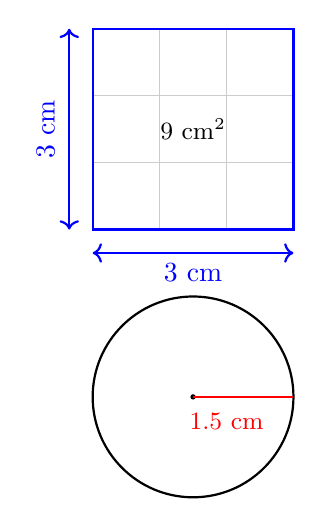
\begin{tikzpicture}[scale=0.85]
  \draw[gray!40, thin] (0,0) grid (3,3);
  \draw[thick, blue] (0,0) rectangle (3,3);
  \draw[blue, thick, <->] (0,-0.35) -- (3,-0.35);
  \node[blue] at (1.5,-0.65) {$3$ cm};
  \draw[blue, thick, <->] (-0.35,0) -- (-0.35,3);
  \node[blue, rotate=90] at (-0.7,1.5) {$3$ cm};
  \node at (1.5,1.5) {\small $9$ cm$^2$};
  % Small circle below for context
  \draw[thick] (1.5,-2.5) circle (1.5cm);
  \fill (1.5,-2.5) circle (0.04);
  \draw[red, thick] (1.5,-2.5) -- ++(0:1.5);
  \node[red, below] at (2,-2.6) {\small $1.5$ cm};
\end{tikzpicture}
\end{center}

\column{0.65\textwidth}
\small
\begin{enumerate}
  \begin{multicols}{2}
    \item $4 \times 4 = $ \ans{$16$}
    \item $7 \times 7 = $ \ans{$49$}
  \end{multicols}
  \begin{multicols}{2}
    \item $10^2 = $ \ans{$100$}
    \item $3^2 = $ \ans{$9$}
  \end{multicols}
  \item \ans{No. $2\times6=12$ but $6^2=36$. Squaring means multiplying by itself.}
  \begin{multicols}{2}
    \item $3.14\times9=$ \ans{$28.26$}
    \item $3.14\times25=$ \ans{$78.5$}
  \end{multicols}
\end{enumerate}
\vspace{-0.5em}
\begin{enumerate}
  \setcounter{enumi}{6}
  \item (a) radius $=$ \ans{$7$ cm} \quad (b) $C = \pi d \approx 3.14\times14=$ \ans{$43.96$ cm}
  \item (a) $C=\pi d\approx3.14\times10=$ \ans{$31.4$ cm}
  \item \ans{Less than $9$ cm$^2$. The circle doesn't fill all four corners of the square.}
\end{enumerate}

\end{columns}
\end{frame}

%------------------------------------------------
% SLIDE 2 SOLUTIONS
%------------------------------------------------
\begin{frame}{Starter --- Solutions}

\begin{columns}

\column{0.35\textwidth}
\begin{center}
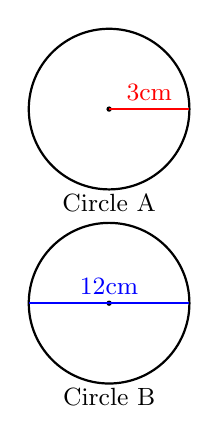
\begin{tikzpicture}[scale=0.85]
  % Circle A — radius labelled
  \draw[thick] (0,2.5) circle (1.2cm);
  \fill (0,2.5) circle (0.04);
  \draw[red, thick] (0,2.5) -- ++(0:1.2);
  \node[red] at (0.6, 2.75) {\small $3$cm};
  \node at (0, 1.1) {\small Circle A};
  % Circle B — diameter labelled
  \draw[thick] (0,-0.4) circle (1.2cm);
  \fill (0,-0.4) circle (0.04);
  \draw[blue, thick] (-1.2,-0.4) -- (1.2,-0.4);
  \node[blue] at (0,-0.15) {\small $12$cm};
  \node at (0,-1.8) {\small Circle B};
\end{tikzpicture}
\end{center}

\column{0.65\textwidth}
\small
\begin{enumerate}
  \begin{multicols}{2}
    \item Halve $12$: \ans{$6$ cm}
    \item Halve $9.4$: \ans{$4.7$ cm}
  \end{multicols}
  \begin{multicols}{2}
    \item $6^2=$ \ans{$36$}
    \item $1.5^2=$ \ans{$2.25$}
    \item $3\times4^2=$ \ans{$48$}
    \item \ans{True. $\pi\times2r = 2\pi r$. }
  \end{multicols}
\end{enumerate}
\vspace{-1.5em}
\begin{enumerate}
  \setcounter{enumi}{6}
  \item Circle A, $r=3$ cm: \newline
    (a) $C=2\pi r\approx2\times3.14\times3=$ \ans{$18.84$ cm} \newline
    (b) $A=\pi r^2\approx3.14\times9=$ \ans{$28.26$ cm$^2$}
  \item Circle B, $d=12$ cm so $r=6$ cm: \newline
    (a) $C=\pi d\approx3.14\times12=$ \ans{$37.68$ cm} \newline
    (b) $A=\pi r^2\approx3.14\times36=$ \ans{$113.04$ cm$^2$}
  \item Circumference ratio: $\frac{37.68}{18.84}=$ \ans{$2$. Yes, double.} \newline
    Area ratio: $\frac{113.04}{28.26}=$ \ans{$4$. No --- area is $\times 4$, not $\times 2$!}
\end{enumerate}

\end{columns}
\end{frame}

%------------------------------------------------
% SLIDE 3 SOLUTIONS
%------------------------------------------------
\begin{frame}{Starter --- Solutions}

\vspace{-1em}

\begin{columns}

\column{0.35\textwidth}
\begin{center}
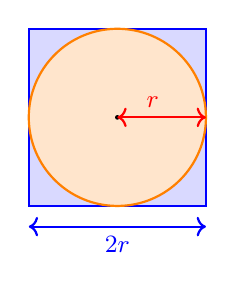
\begin{tikzpicture}[scale=0.75]
  \begin{scope}
    \clip (0,0) rectangle (3,3);
    \fill[blue!15] (0,0) rectangle (3,3);
    \fill[orange!20] (1.5,1.5) circle (1.5cm);
  \end{scope}
  \draw[thick, blue] (0,0) rectangle (3,3);
  \draw[thick, orange] (1.5,1.5) circle (1.5cm);
  \fill (1.5,1.5) circle (0.04);
  \draw[red, thick, <->] (1.5,1.5) -- ++(0:1.5);
  \node[red] at (2.1,1.75) {\small $r$};
  \draw[blue, thick, <->] (0,-0.35) -- (3,-0.35);
  \node[blue] at (1.5,-0.65) {\small $2r$};
\end{tikzpicture}
\end{center}

\column{0.65\textwidth}
\small
\begin{enumerate}
  \begin{multicols}{2}
    \item $5\times5=$ \ans{$25$}
    \item $8^2=$ \ans{$64$}
  \end{multicols}
  \begin{multicols}{2}
    \item $2.5^2=$ \ans{$6.25$}
    \item $3.14\times9=$ \ans{$28.26$}
  \end{multicols}
  \item $7\times4=$ \ans{$28$ cm$^2$}
  \item \ans{$\frac{1}{4}$ of $360^\circ$. And $\frac{3}{4}$.}
\end{enumerate}

\begin{enumerate}
  \setcounter{enumi}{6}
  \item Area of circle $=$ \ans{$\pi r^2$}
  \item Shaded area $=$ area of square $-$ area of circle $=$ \ans{$(2r)^2 - \pi r^2 = 4r^2 - \pi r^2$}
  \item Perimeter $48$ cm $\Rightarrow$ side $= 12$ cm $\Rightarrow r = 6$ cm. \newline
    Square area $= 12^2 =$ \ans{$144$ cm$^2$} \newline
    Circle area $= \pi\times6^2\approx3.14\times36=$ \ans{$113.04$ cm$^2$} \newline
    Shaded area $\approx144-113.04=$ \ans{$30.96$ cm$^2$}
\end{enumerate}

\end{columns}
\end{frame}

% WIP

% %------------------------------------------------
% % SLIDE 4 SOLUTIONS
% %------------------------------------------------
% \begin{frame}{Starter --- Solutions}

% \vspace{-1em}

% \begin{columns}

% \column{0.35\textwidth}
% \begin{center}
% \begin{tikzpicture}[scale=0.85]
%   \draw[thick] (0, 2.2) circle (0.8cm);
%   \fill[red!15] (0,2.2) circle (0.8cm);
%   \fill (0,2.2) circle (0.04);
%   \draw[red, thick] (0,2.2) -- ++(0:0.8);
%   \node[red] at (0.4, 2.45) {\small $4$};
%   \node at (0, 1.2) {\small Circle P};
%   \draw[thick] (0,-0.4) circle (1.4cm);
%   \fill[blue!15] (0,-0.4) circle (1.4cm);
%   \fill (0,-0.4) circle (0.04);
%   \draw[blue, thick] (-1.4,-0.4) -- (1.4,-0.4);
%   \node[blue] at (0,-0.15) {\small $d=14$};
%   \node at (0,-2.0) {\small Circle Q};
%   \node[gray] at (0,-2.45) {\small (cm)};
% \end{tikzpicture}
% \end{center}

% \column{0.65\textwidth}
% \small
% \begin{enumerate}
%   \begin{multicols}{2}
%     \item $9^2=$ \ans{$81$}
%     \item $3.5^2=$ \ans{$12.25$}
%   \end{multicols}
%   \begin{multicols}{2}
%     \item $3.14\times16=$ \ans{$50.24$}
%     \item $3.14\times49=$ \ans{$153.86$}
%   \end{multicols}
%   \item Halve $14=7$. $\;7^2=$ \ans{$49$}
%   \item Side $=$ \ans{$8$ cm} \quad ($8^2=64$)
% \end{enumerate}

% \begin{enumerate}
%   \setcounter{enumi}{6}
%   \item \ans{The mistake: diameter was used instead of radius. $r=7$ cm, so $A=\pi\times7^2\approx3.14\times49\approx153.86$ cm$^2$.}
%   \item Circle P, $r=4$ cm: \newline
%     (a) $A=\pi\times4^2\approx3.14\times16=$ \ans{$50.24$ cm$^2$} \newline
%     (b) $C=\pi d\approx3.14\times8=$ \ans{$25.12$ cm}
%   \item Circle Q, $d=14\Rightarrow r=7$ cm: \newline
%     (a) $A=\pi\times7^2\approx$ \ans{$153.86$ cm$^2$} \newline
%     (b) $C=\pi d\approx3.14\times14=$ \ans{$43.96$ cm}
%   \item \ans{Circle Q is larger. Difference $\approx153.86-50.24=103.62$ cm$^2$.}
% \end{enumerate}

% \end{columns}
% \end{frame}

\end{document}